%--------------------------------------------------------------------------------------------------
% Präsentation ICC-System:
%		Stand der Dinge in Sachen Rückkopplungskompensation und Ausblick
%
%--------------------------------------------------------------------------------------------------


\section{System Design, Training and Testing}

%~~~~~~~~~~~~~~~~~~~~~~~~~~~~~~~~~~~~~~~~~~~~~~~~~~~~~~~~~~~~~~~~~~~~~~~~~~~~~~~~~~~~~~~~~~~~~~~~~~
% New subsection
%~~~~~~~~~~~~~~~~~~~~~~~~~~~~~~~~~~~~~~~~~~~~~~~~~~~~~~~~~~~~~~~~~~~~~~~~~~~~~~~~~~~~~~~~~~~~~~~~~~
\subsection{Feature Extraction}

%--------------------------------------------------------------------------------------------------
% New frame
%--------------------------------------------------------------------------------------------------
\begin{frame}{\insertsection}{\insertsubsection}   
 \headline{Possible problems}
\begin{itemize}
\uncover<1->{
\item Pitch}
\uncover<2->{
\item Different speakers (absolut output value)}
\uncover<3->{
\item Noise}
\end{itemize}

\only<4->{
\headline{Continuous feature vectors}
\medskip
\begin{itemize}
\uncover<4->{
\item 13 MFCC (Mel-frequency cepstrum coefficients)}
\uncover<5->{
\item 26 dynamical features (independent of absolute value)}
\uncover<6->{
\item 30 ms time frame}
\end{itemize}}




 \end{frame}
 
  \subsection{HMM}
 %--------------------------------------------------------------------------------------------------
% New frame
%--------------------------------------------------------------------------------------------------
\begin{frame}{\insertsection}{\insertsubsection}   
 \medskip
\headline{Number of States for left-right HMM}
\begin{itemize}
\uncover<1->{
\item Trade off: too few parameters vs. amount of training data}
\uncover<2->{
\item Also: Limited training data}
\uncover<3->{
\item State assignment due to syllables + start/end state}

\end{itemize}
\vspace{5mm}
\only<4->{
\begin{columns}
\column{0.4\textwidth}
\textit{environmnent}: 6 states
\column{0.5\textwidth}
\textit{chair}: 4 states
\end{columns}}
\vspace{5mm}
\only<5->{
\headline{Output distributions}
\begin{itemize}
\item GMM (Gaussian Mixture Models)
\end{itemize}}




 
 \end{frame}
 
\subsection{Training data and validation set}
 %--------------------------------------------------------------------------------------------------
% New frame
%--------------------------------------------------------------------------------------------------
\begin{frame}{\insertsection}{\insertsubsection}   
 \headline{Recorded data}
 \begin{itemize}
 \uncover<1->{
 \item 5 people: 15 recordings per word
 \item One person has been disregarded
 \item 840 recordings in total, 60 per word}
 \end{itemize}
 \vspace{8mm}
 \only<2->{
\headline{k-fold approach}
 \begin{itemize}
 \item k=5 sets
 \item 48 training and 12 validation samples
 \end{itemize}}

 
 \end{frame}
 

 
  \subsection{Testing and tweaking}
 %--------------------------------------------------------------------------------------------------
% New frame
%--------------------------------------------------------------------------------------------------
\begin{frame}{\insertsection}{\insertsubsection}   
 
\headline{Final HMM}
 \begin{itemize}
 \uncover<1->{
 \item 5 sets have been tweaked on their validation set and compared on the whole set.}
  \uncover<2->{
 \item Recognition rate in table below}
 \end{itemize}
 \only<3->{
\begin{tabular}{c |c c c c c c c}
word& 1 & 2 & 3 & 4 & 5 & 6 & 7 \\
\hline
validation set & 1.00 & 1.00& 1.00 & 1.00 & 1.00& 1.00& 1.00\\
overall &0.76 &0.95 & 1.00 &1.00&1.00&1.00&1.00\\
\hline
\hline
word & 8 & 9 & 10 & 11 & 12 & 13 & 14\\
\hline
validation set & 1.00& 1.00& 1.00& 0.833& 1.00& 1.00& 1.00\\
overall &1.00&0.95&1.00&0.7&1.00&0.95&1.00\\
\end{tabular}}
 \end{frame}
 
 \begin{frame}{\insertsection}{\insertsubsection}   
 \headline{Some realizations}
   \only<1>{
 \begin{itemize}
 \item word \textit{I} and 1st MFCC coefficient
 \end{itemize}
\vspace{0mm}
\begin{center}
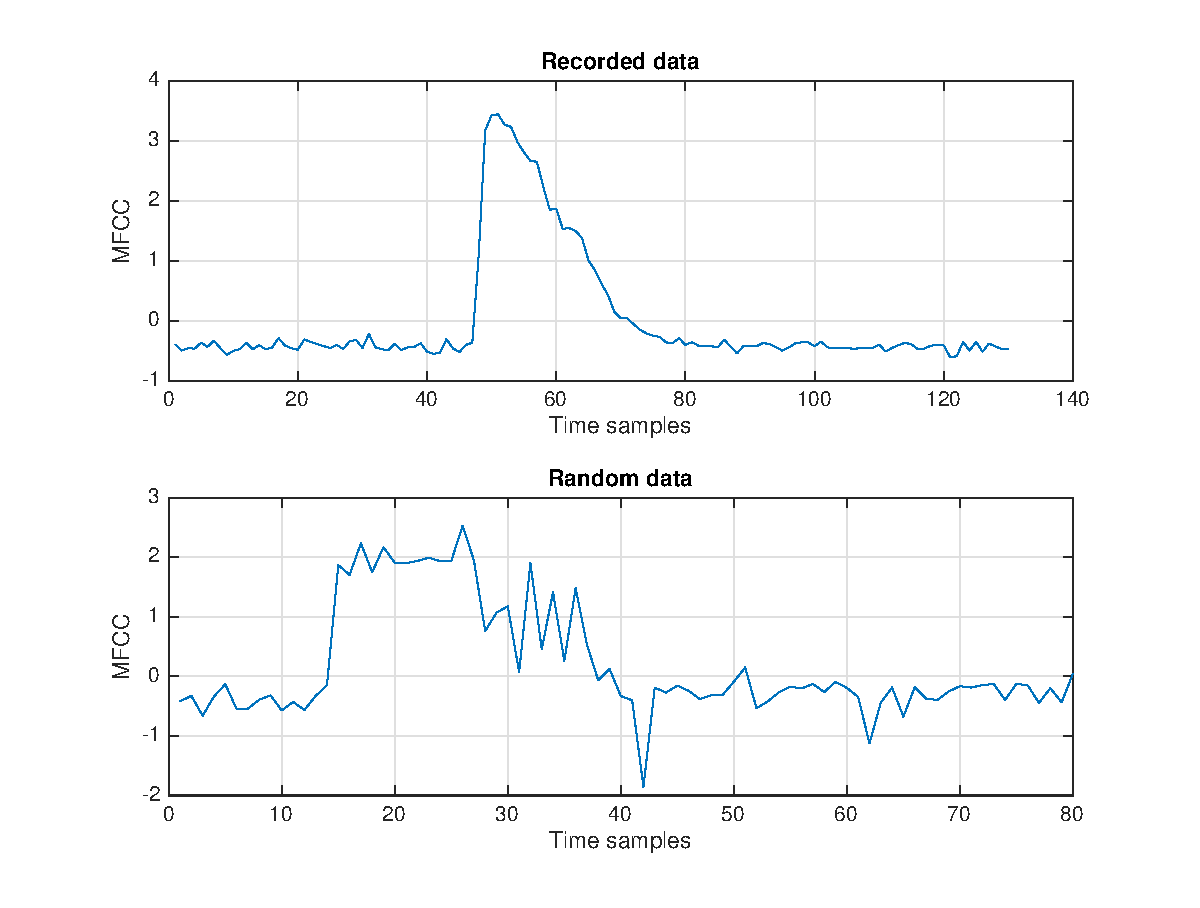
\includegraphics[width=0.65\textwidth]{figures/example}
\end{center}}
  \only<2>{
  \begin{itemize}
 \item word \textit{I} and 2nd MFCC coefficient
 \end{itemize}
\vspace{0mm}
\begin{center}
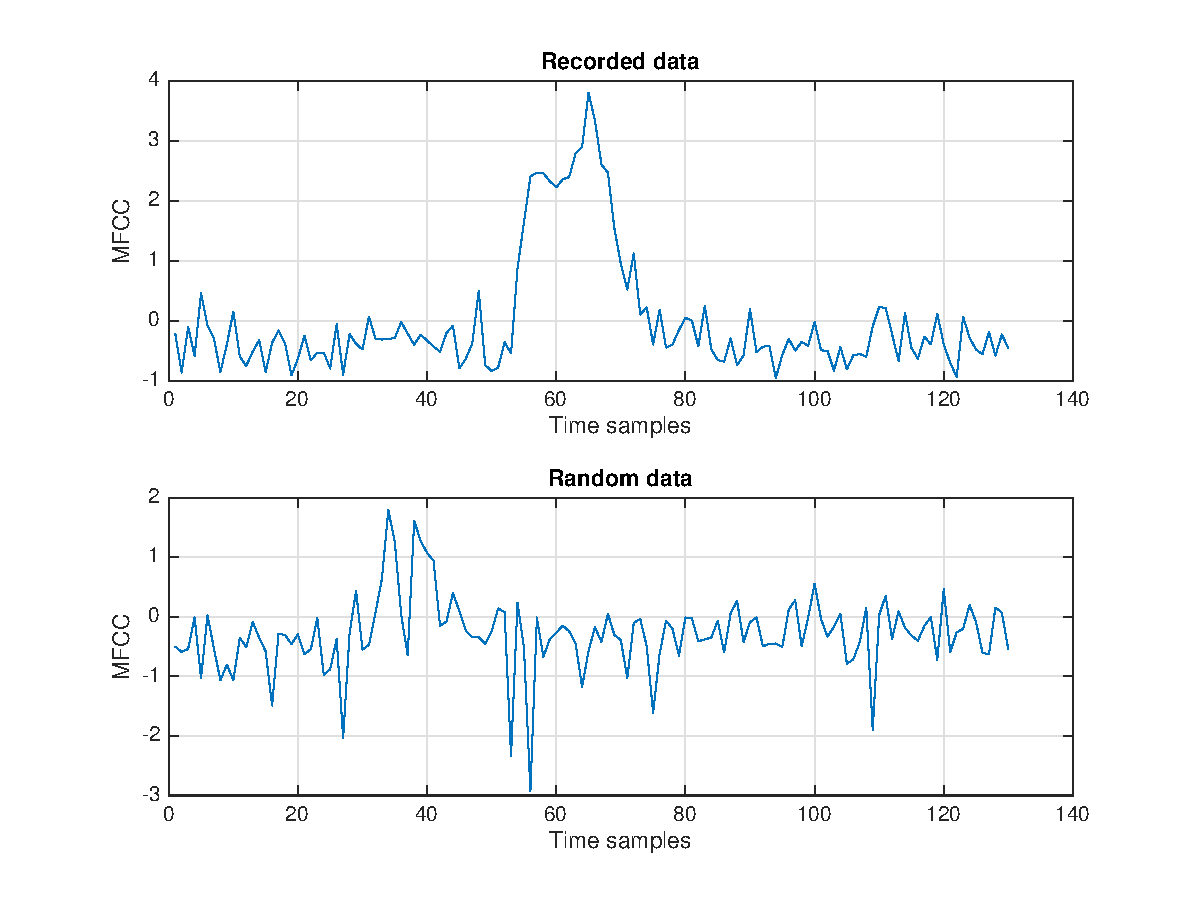
\includegraphics[width=0.65\textwidth]{figures/example2}
\end{center}}
 \end{frame}
 

 
%  \subsection{Varying Time Delay}
% %--------------------------------------------------------------------------------------------------
%% New frame
%%--------------------------------------------------------------------------------------------------
%\begin{frame}{\insertsection}{\insertsubsection}   
% 
%\headline{Varying Time Delay}
%\medskip
%\begin{itemize}
%	\uncover<2->{
%	\item  Dead-time sensitivity of MPC}
%	\uncover<3->{
%	\item  Possible Problem: Prediction horizone of MPC}
%	\uncover<4->{
%	\item MPC quality degrades if error between used model and real time delay increases}
%\end{itemize}
%
%\uncover<5->{
%\begin{block} \centering
%	Varying time delay results in the need of a \headline{robust} controller. Several possible solutions mentioned in papers...
%\end{block}
%}
 
% \end{frame}
 
 

 


 